% Springer Nature manuscript prepared from the team's supplied project records and result archives.
% A public repository URL will be added after the final GitHub upload.
\PassOptionsToPackage{hypertexnames=false}{hyperref}
\documentclass[pdflatex,sn-mathphys-num]{sn-jnl}

\usepackage{graphicx}
\usepackage{multirow}
\usepackage{amsmath,amssymb,amsfonts}
\usepackage{booktabs}
\usepackage{array}
\usepackage{url}
\usepackage{hyperref}
\hypersetup{
  pdftitle={Trace-Driven Comparative Evaluation of Threshold and Reinforcement-Learning Controllers for Horizontal Cloud Auto-Scaling},
  pdfauthor={Dilshad; Utkarsh; Saurabh Verma},
  pdfsubject={Trace-driven evaluation of horizontal cloud auto-scaling controllers},
  pdfkeywords={cloud auto-scaling, SARSA, Q-learning, CloudSim Plus, Bitbrains workload traces}
}
\usepackage{algorithm}
\usepackage{algpseudocode}
\usepackage{enumitem}
\usepackage{siunitx}
\graphicspath{{figures/}}
\raggedbottom

\newcommand{\method}{S-Threshold+SARSA}
\newcommand{\qmethod}{Q-Threshold}
\newcommand{\cloudsim}{CloudSim Plus}

\begin{document}

\title[Trace-driven evaluation of cloud auto-scaling controllers]{Trace-Driven Comparative Evaluation of Threshold and Reinforcement-Learning Controllers for Horizontal Cloud Auto-Scaling}

% Author names, order, and institutional email addresses supplied by the team.
% Dilshad is the corresponding author.
\author*[1]{\fnm{Dilshad}}\email{dilshad.ug24@nsut.ac.in}
\author[1]{\fnm{Utkarsh}}\email{utkarsh_ug24@nsut.ac.in}
\author[1]{\fnm{Saurabh} \sur{Verma}}\email{saurabh.verma.ug24@nsut.ac.in}

\affil*[1]{\orgdiv{Department of Information Technology}, \orgname{Netaji Subhas University of Technology}, \orgaddress{\city{New Delhi}, \country{India}}}

\abstract{Horizontal auto-scaling adjusts the number of virtual machines (VMs) as workload changes. This study compares four controllers in CloudSim Plus: fixed allocation (STATIC), CPU-threshold scaling (THRESHOLD\_ONLY), threshold-gated SARSA (S-THRESHOLD\_SARSA), and a Q-learning threshold variant (Q-THRESHOLD). The workload is derived from 1,250 VM files in the fastStorage portion of the GWA-T-12 Bitbrains trace. We aggregate 8,640 five-minute observations over 30 days and apply one global 95th-percentile (P95) CPU calibration, mapping that reference to 90\% of a ten-VM baseline capacity. Normalized offered load is converted into staggered synthetic CloudSim Plus Cloudlet arrivals; the original applications are not replayed. Across 30 valid daily aggregates, adaptive controllers reduce mean response time relative to STATIC. S-THRESHOLD\_SARSA has the lowest mean and P95 response times, while Q-THRESHOLD records fewer VM-seconds and fewer scaling-direction reversals. The findings indicate a latency, resource-use, and stability trade-off. Implementation assumptions and reproducibility limitations are reported.}

\keywords{Cloud computing, horizontal auto-scaling, reinforcement learning, SARSA, Q-learning, workload traces, CloudSim Plus, resource management}

\maketitle

\section{Introduction}\label{sec:intro}

Cloud computing provides on-demand access to processing, storage, and network resources. An important advantage of this model is elasticity: the amount of provisioned capacity can be increased when demand rises and reduced when demand falls. For a cloud-hosted application, however, the demand for computing resources is rarely constant. Workload intensity can vary across time, and a fixed resource allocation may therefore be inefficient. A pool that is too small can create queues and increase task response time; a pool that is too large can consume resources without a corresponding performance benefit. Auto-scaling attempts to balance these competing effects by adjusting the provisioned capacity in response to observed workload conditions \cite{qu2018autoscaling,machiraju2026survey}.

Horizontal auto-scaling changes the number of running instances, such as virtual machines (VMs), while vertical scaling changes the capacity assigned to an existing instance. This study concentrates on horizontal scaling. The controller considered here observes CPU utilization and selects one of three actions: scale out, scale in, or take no action. These choices appear simple, but the controller must balance responsiveness against unnecessary changes. A controller that scales out too late can allow response times to increase. A controller that reacts to every small fluctuation can repeatedly add and remove VMs, a behavior referred to in this study as scaling flapping.

Threshold-based policies are attractive because they are easy to interpret and inexpensive to execute. They compare a monitored metric with one or more configured bounds and trigger scaling when a bound is crossed. Their limitation is that a fixed threshold policy does not explicitly learn from the observed consequences of previous decisions. Reinforcement learning (RL) offers an alternative: an agent observes a state, chooses an action, receives feedback, and updates its action-value estimates. The selected base study by Archana and Kumar combines a threshold model with the State--Action--Reward--State--Action (SARSA) algorithm to perform horizontal auto-scaling \cite{archana2025sthreshold}.

The present work implements the core threshold-plus-SARSA idea in \cloudsim{} and extends its evaluation to a 30-day trace-derived workload. The experiment compares four modes under a common trace-calibration policy: STATIC, THRESHOLD\_ONLY, S-THRESHOLD\_SARSA, and Q-THRESHOLD. The first two modes act as baselines. The third is the implementation derived from the selected S-Threshold paper. The fourth is a separate project-level Q-learning threshold variant with additional stabilization settings recorded in its experiment configuration. It is not presented as a second implementation of the same SARSA algorithm.

The study is designed to answer three questions:
\begin{enumerate}[label=\textbf{RQ\arabic*.},leftmargin=2.0em]
  \item How do static, threshold-only, and learning-based controllers compare in response time, P95 response time, waiting time, makespan, throughput, and resource consumption under the same trace-derived offered workload?
  \item Does the threshold-gated SARSA controller reduce scaling-direction reversals relative to threshold-only scaling?
  \item What trade-off does the Q-THRESHOLD project variant exhibit relative to S-THRESHOLD\_SARSA in latency, VM-seconds, and scaling stability?
\end{enumerate}

The contributions of this study are experimental and implementation-oriented rather than a claim of a newly invented RL algorithm. First, the work creates a common trace-derived workload from 1,250 Bitbrains fastStorage VM files and applies a single global P95-based calibration across 30 days. Second, it implements the S-Threshold/SARSA decision flow in a CloudSim Plus simulation, including threshold gating of SARSA-selected actions, VM-bound checks, safe scale-in, and reassignment of future Cloudlets. Third, it evaluates four controller modes using a set of latency, throughput, resource-use, and stability metrics. Fourth, it makes implementation assumptions and reproducibility caveats explicit so that the measured results are not confused with a literal replication of every detail in the reference paper.

The remainder of the paper is organized as follows. Section~\ref{sec:related} reviews related work. Section~\ref{sec:background} describes the system model and controller concepts. Section~\ref{sec:method} presents the trace preparation, simulation configuration, controller modes, and measurement definitions. Section~\ref{sec:implementation} explains the implementation flow. Section~\ref{sec:results} reports the experimental results, and Section~\ref{sec:discussion} discusses their interpretation and limitations. Section~\ref{sec:conclusion} concludes the paper.

\section{Related Work}\label{sec:related}

\subsection{Cloud elasticity and threshold-based auto-scaling}

Cloud elasticity allows a service to provision and release resources as demand changes. Qu et al. provide a widely cited taxonomy and survey of cloud auto-scaling methods, discussing the design choices and challenges associated with scaling web applications while satisfying quality-of-service (QoS) requirements \cite{qu2018autoscaling}. Their review highlights that auto-scaling is not defined only by the rule that triggers an action: it also depends on the monitored metrics, control interval, scaling granularity, application architecture, and the relationship between resource cost and service performance.

A threshold controller is a reactive policy. It monitors a metric such as CPU utilization and compares the measured value with configured boundaries. A high value can trigger scale-out, while a low value can trigger scale-in. Kubernetes Horizontal Pod Autoscaling illustrates the continued practical relevance of metric-driven horizontal control: its controller periodically compares observed resource metrics with a target and adjusts the desired number of replicas \cite{kubernetesHPA}. Threshold control is understandable and operationally simple, but static bounds may not represent every workload pattern or service condition. The 2026 systematic review by Machiraju et al., which classifies 60 primary studies published from 2015 to 2025, identifies workload variation, delayed actuation, multi-objective optimization, and the fragmented nature of evaluation frameworks as continuing challenges for ML-based auto-scaling \cite{machiraju2026survey}.

Threshold-based methods remain important as baselines even when more complex controllers are proposed. They provide a clear reference point for asking whether an adaptive method actually improves outcomes. The present study therefore includes THRESHOLD\_ONLY as a separate mode rather than comparing only learning-based methods.

\subsection{Reinforcement learning for cloud resource management}

Reinforcement learning models a sequential decision process in which an agent selects actions and receives rewards from an environment. Qiu et al. present AWARE, a framework for applying reinforcement learning to workload auto-scaling in production cloud systems. Their work focuses on practical concerns including adaptation to different workloads and safe exploration, illustrating that the transition from an RL algorithm to a dependable cloud controller involves more than selecting a learning rule \cite{qiu2023aware}.

Song et al. propose a Q-learning-based auto-scaling approach for provisioning big-data analysis services in cloud environments. Their study is relevant because it uses Q-learning to address the relationship between resource utilization and cost in a cloud provisioning problem \cite{song2024qlearning}. Q-learning and SARSA are both temporal-difference control methods, but their update targets differ: SARSA uses the value of the next action selected by the current policy, whereas Q-learning uses the maximum estimated value among next-state actions. This distinction motivates examining a Q-learning threshold variant separately from the SARSA-based controller.

Recent work has also combined prediction with reinforcement learning. Lipari et al. describe a Kubernetes-oriented approach that combines an LSTM workload forecaster with a deep Q-network to adjust container replicas proactively \cite{lipari2025forecast}. The method represents a predictive direction, whereas the controllers evaluated in this study are reactive to the CPU signal and task queue observed during the simulation. The 2026 survey by Machiraju et al. further discusses predictive, hybrid horizontal--vertical, and policy-optimization approaches, while identifying multi-objective cost, QoS, and energy management as open evaluation challenges \cite{machiraju2026survey}.

\subsection{Selected S-Threshold study and positioning of this work}

The selected base paper is ``A S-Threshold Method to Perform Horizontal Auto-Scaling in a Cloud Computing Environment'' by Archana and Kumar \cite{archana2025sthreshold}. The authors combine threshold-based workload states with SARSA. The proposed design initially uses threshold rules to guide decisions and then uses experience-based updates to adapt action preferences. The article reports CloudSim Plus experiments involving different numbers of Cloudlets, processing speeds, and VMs, and discusses makespan, response time, waiting duration, average turnaround time, and throughput \cite{archana2025sthreshold}.

The current project follows the paper's core idea of combining workload states, threshold guidance, and SARSA action-value learning. It does not claim a line-by-line reproduction. Some details in the paper require interpretation or are not fully specified. In particular, the paper discusses CPU and memory in its workload description but does not provide a complete formula for combining them into one state variable. Its prose refers to dynamic thresholds, while its pseudocode gives fixed 30\% and 70\% values without a complete adaptation rule. The reward description also creates an ambiguity: the objective is to minimize response time, whereas the pseudocode states the response time itself as the reward in a reward-maximizing SARSA procedure. The implementation choices adopted for this study are documented in Section~\ref{subsec:sarsa}.

The 30-day experiment in this paper should be understood as an additional trace-driven behavior study. It is distinct from the synthetic parameter-sweep benchmark in the base paper. The trace-derived workload is transformed into staggered synthetic Cloudlet arrivals, and the same arrival sequence is supplied to the compared modes. Consequently, the present results characterize the behavior of these simulated controllers under a calibrated trace-derived offered load; they are not production-cloud measurements and do not reproduce the original Bitbrains application execution.

\subsection{Research gap and study focus}

The literature indicates continuing interest in adaptive resource management, but comparison remains difficult when studies use different workloads, simulators, metrics, and controller assumptions \cite{qu2018autoscaling,machiraju2026survey}. This work addresses a narrower experimental question: under one shared trace-derived workload and one CloudSim Plus infrastructure, how do a fixed pool, a reactive threshold controller, a threshold-gated SARSA controller, and a stabilized Q-learning threshold variant differ in latency, resource use, and scaling reversals? The goal is not to assert that one controller is universally superior. Instead, the evaluation reports the trade-offs observed under the stated configuration and makes the workload transformation and implementation limitations reproducible.

\section{System Model and Controller Background}\label{sec:background}

\subsection{Horizontal auto-scaling model}

Let the simulated VM pool at decision time $t$ contain $N_t$ active VMs. The controller observes a CPU-utilization signal $u_t$ and selects an action from the set
\begin{equation}
  \mathcal{A}=\{\text{SCALE\_OUT},\text{SCALE\_IN},\text{NO\_ACTION}\}.
  \label{eq:actions}
\end{equation}
The available actions are given in Eq.~\ref{eq:actions}. A scale-out action adds one VM, a scale-in action removes one eligible VM, and no-action leaves the pool unchanged. The project bounds the active VM count by $N_{\min}=2$ and $N_{\max}=40$. These bounds prevent the policy from requesting a pool size outside the configured simulation capacity.

The STATIC mode fixes the pool at ten VMs. THRESHOLD\_ONLY uses the same low/high CPU boundaries as the S-Threshold controller but applies the threshold action directly. The S-THRESHOLD\_SARSA mode classifies CPU utilization into threshold-defined states, lets SARSA select from all three scaling actions, and then applies a separate threshold gate before checking whether the corresponding VM operation is feasible. The Q-THRESHOLD mode is a separate Q-learning threshold controller; its recorded experiment configuration includes additional mechanisms intended to smooth or delay scaling decisions.

\subsection{Workload state and threshold interpretation}

For the trace-based S-Threshold path, average CPU utilization across executing CloudSim VMs is classified into three workload states:
\begin{equation}
S_t=\begin{cases}
\text{LOW}, & u_t < 30\%,\\
\text{MEDIUM}, & 30\%\leq u_t\leq70\%,\\
\text{HIGH}, & u_t>70\%.
\end{cases}
\label{eq:states}
\end{equation}
The threshold recommendation is SCALE\_IN for LOW, NO\_ACTION for MEDIUM, and SCALE\_OUT for HIGH. In the v78 trace implementation, the SARSA agent first selects an action from the complete action set $\{\text{SCALE\_IN},\text{SCALE\_OUT},\text{NO\_ACTION}\}$ using epsilon-greedy selection. A separate threshold gate then accepts the selected action only when it agrees with the threshold direction: LOW accepts SCALE\_IN, HIGH accepts SCALE\_OUT, and MEDIUM always returns NO\_ACTION. Thus, an action selected by SARSA can be converted to NO\_ACTION by the threshold gate. The agent's selected action is retained for the SARSA transition; it is not replaced by the threshold-gated or physically applied action.

This is a fixed-threshold implementation. Although the base paper's discussion mentions dynamic thresholds, the available description does not provide a complete rule for adapting both thresholds over time. Accordingly, the present S-Threshold implementation does not claim to implement an unspecified adaptive-threshold mechanism.

\subsection{SARSA action-value learning}

SARSA is an on-policy temporal-difference method. For a state $s_t$, action $a_t$, reward $r_{t+1}$, next state $s_{t+1}$, and next action $a_{t+1}$, the action-value update is
\begin{equation}
Q(s_t,a_t)\leftarrow Q(s_t,a_t)+\alpha\left[r_{t+1}+\gamma Q(s_{t+1},a_{t+1})-Q(s_t,a_t)\right],
\label{eq:sarsa}
\end{equation}
where $\alpha$ is the learning rate and $\gamma$ is the discount factor \cite{sutton2018reinforcement}. The implementation uses $\alpha=0.1$, $\gamma=0.9$, and $\epsilon=0.1$ for epsilon-greedy action selection. These numeric values are project configuration choices; they are not claimed to be values supplied by the selected base paper.

The agent explores with probability $\epsilon=0.1$ and otherwise selects the action with the highest estimated Q-value. The Q-table stores values for each LOW, MEDIUM, and HIGH state and each of the three scaling actions. When several actions have the same initial Q-value, the implementation's default choice is SCALE\_IN for LOW, SCALE\_OUT for HIGH, and NO\_ACTION for MEDIUM. During exploration, however, the random choice is drawn from all three actions; the subsequent threshold gate determines whether that choice can trigger a VM change.

\subsection{Reward design and interpretation}

The v78 trace runner computes the SARSA reward from the broker's waiting-list backlog, not from measured response time. Let $B_t$ denote the number of Cloudlets in the waiting list at a controller observation. The reward supplied to the SARSA transition is
\begin{equation}
r_t=\frac{1}{B_t+1}.
\label{eq:reward}
\end{equation}
The implementation obtains this value by calling the reciprocal reward function with the waiting-list size plus one. A smaller waiting backlog therefore yields a larger reward. Response time is measured separately as an evaluation metric; it is not the S-Threshold SARSA reward in the selected v78 trace experiment. The reward is a project implementation choice and should not be described as a direct implementation of an ambiguously specified response-time reward in the reference paper.

\subsection{Q-learning threshold control}

Q-learning is an off-policy temporal-difference method. In its usual tabular form, its update uses the maximum estimated value of the next state, as shown in Eq.~\ref{eq:qlearning}:
\begin{equation}
Q(s_t,a_t)\leftarrow Q(s_t,a_t)+\alpha\left[r_{t+1}+\gamma\max_{a'}Q(s_{t+1},a')-Q(s_t,a_t)\right].
\label{eq:qlearning}
\end{equation}
The Q-THRESHOLD mode is a separate project variant that uses Q-learning to adjust threshold decisions. The output configuration supplied with the stabilized-v2 results records an exponential moving-average CPU signal, queue-aware scale-out, two consecutive scale-out samples, four consecutive scale-in samples, a 30-second threshold-adjustment interval, a 10-second minimum action gap, and a 45-second scale-in hold following confirmed scale-out, and a 45-second retry backoff after VM-allocation failure. The experiment uses $\alpha=0.1$, $\gamma=0.9$, and $\epsilon=0.1$. Its reward is described in the run configuration as a project-level reward based on response time and VM count; it is not presented as the exact reward formula of another published Q-Threshold algorithm.

The Q-THRESHOLD description is based on the `QThreshold-CloudSim-Plus-30Day-Stability-Fix` source archive and the `Q-Threshold-Stabilized-v2` result signature. The inspected source contains the recorded EMA, queue-aware scale-out, consecutive-sample confirmation, action-gap, scale-in-hold, and allocation-retry mechanisms. The source settings are consistent with the supplied result configuration. However, the historical result package does not record a source commit hash or executable build hash; exact binary provenance therefore cannot be established retrospectively.

\section{Experimental Methodology}\label{sec:method}

\subsection{Trace source and workload characteristics}

The workload source is the GWA-T-12 Bitbrains fastStorage trace. The Grid Workloads Archive describes GWA-T-12 as a collection of anonymized VM performance measurements from a distributed datacenter. The fastStorage subset contains 1,250 VM trace files; the broader dataset also includes a separate Rnd subset \cite{shen2015bitbrains}. The trace provides timestamped measurements including CPU usage, memory, disk, and network-related fields. The present experiment uses the CPU-usage percentage field and does not combine the other resource metrics into the workload state.

The selected input directory contains 1,250 CSV files for the fastStorage month used in the run. The loader identifies columns by header name, aligns observations using timestamp-derived step indices, and averages the CPU percentage values reported by VMs in each bucket. Empty time buckets are forward-filled using the most recently observed aggregate value. The processed trace contains 8,641 samples. The experiment uses 8,640 samples, corresponding to 30 days with 288 samples per day; the trailing endpoint sample is excluded.

\subsection{Global P95 workload calibration}

The mean CPU value across the 8,640 simulated samples is 7.2054\%, and the global P95 is 12.4129\%. The global P95 is calculated once across the complete 30-day trace rather than independently for each day. The experiment maps this reference value to 90\% of the baseline pool capacity. Let $c_i$ denote the aggregated CPU percentage at trace step $i$, and let $P_{95}$ denote the global 95th-percentile value. The calibration factor is
\begin{equation}
\lambda=\frac{0.90\times100}{P_{95}}=\frac{90}{12.4129}\approx7.25055.
\label{eq:scale}
\end{equation}
Using the calibration factor in Eq.~\ref{eq:scale}, the offered-load fraction supplied to the workload generator is
\begin{equation}
L_i=\frac{c_i}{100}\lambda.
\label{eq:offeredload}
\end{equation}
Equation~\ref{eq:offeredload} applies this shared calibration to each aggregated CPU sample. Consequently, the global P95 sample is mapped to an offered load of approximately 0.90 relative to the capacity of the ten-VM baseline pool. The same $\lambda$ is applied to every day. This is a modelling and calibration choice intended to keep all controller modes on a common workload scale; it does not mean that the original Bitbrains VMs operated at 90\% CPU.

Figure~\ref{fig:p95} summarizes this mapping. The calibration avoids recomputing a separate scale for each day, which would otherwise change the relative meaning of the workload between days. The target value of 90\% is an experiment setting, not a universal definition of P95 or an empirically established optimum. The original and scaled workload values are retained in the experiment outputs.

\begin{figure}[t]
\centering
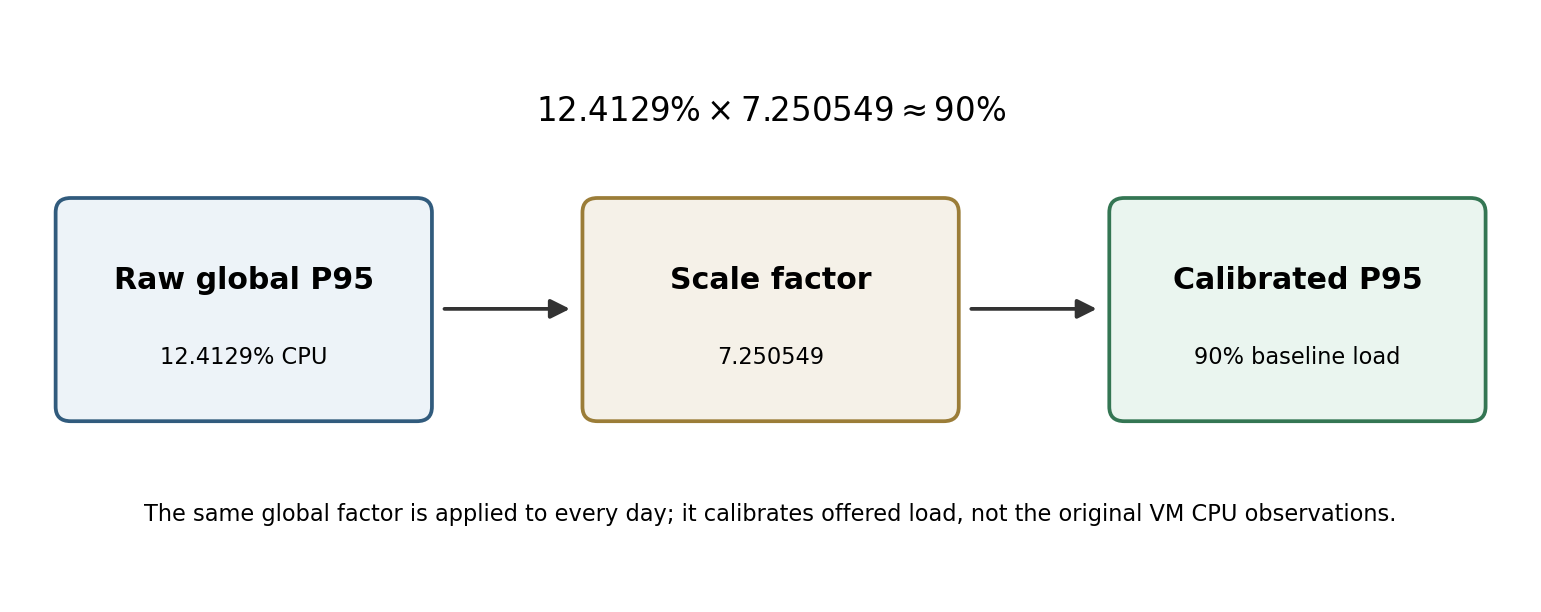
\includegraphics[width=0.88\textwidth]{p95_calibration.png}
\caption{Global P95-based workload calibration. One reference P95 from the full trace is mapped to 90\% of the baseline VM-pool capacity, and the same scale factor is applied to all simulated days.}
\label{fig:p95}
\end{figure}

\subsection{Trace-to-Cloudlet transformation}

The trace observations are not application requests and do not directly identify the original per-VM tasks. To create an executable workload in CloudSim Plus, each 10-second simulated trace window is translated into a number of synthetic Cloudlets. The baseline pool consists of ten VMs, each with 750 million instructions per second (MIPS), and each Cloudlet has a length of 1,000 million instructions (MI). The baseline amount of Cloudlet work corresponding to one trace step is
\begin{equation}
C_{\mathrm{step}}=\frac{N_{\mathrm{base}}\,M\,\Delta t}{\ell}
=\frac{10\times750\times10}{1000}=75,
\label{eq:cloudletcapacity}
\end{equation}
where $N_{\mathrm{base}}=10$ is the baseline VM count, $M=750$ MIPS is the VM processing rate, $\Delta t=10$ seconds is the simulated trace-window duration, and $\ell=1000$ MI is the Cloudlet length. Using the per-window baseline workload in Eq.~\ref{eq:cloudletcapacity}, the expected number of Cloudlets in step $i$ is $L_i C_{\mathrm{step}}$. Fractional Cloudlet counts are carried into the next step so that the cumulative amount of requested work is preserved. Integer Cloudlet arrivals are staggered within each trace window rather than submitted all at once.

This transformation is an important modelling boundary. The end-to-end workload-generation and simulation pipeline is summarized in Fig.~\ref{fig:workflow}. Bitbrains CPU observations determine the amount and timing of offered work; CloudSim Plus then executes synthetic Cloudlets and produces the VM CPU utilization observed by the autoscaling controller. The experiment is therefore trace-driven, but it is not a direct replay of each original VM's execution or a measurement of the original hosted applications.

\subsection{CloudSim Plus infrastructure}

The simulation is implemented in Java using CloudSim Plus 7.2.0. CloudSim Plus supports modelling datacenters, hosts, VMs, task scheduling, and dynamic simulation elements \cite{silvafilho2017cloudsimplus}. The datacenter contains six physical hosts, with four processing elements (PEs) per host. Each PE is configured at 100,000 MIPS. Each host has 11,048 MB RAM, 150,000 bandwidth units, and 1,000,000 storage units. Host-level VM scheduling uses a time-shared policy.

Each VM has one PE, 750 MIPS, 512 MB RAM, 1,000 bandwidth units, and 1,000 storage units. VM-level Cloudlet scheduling uses a space-shared policy. The pool starts with ten VMs and is bounded between two and forty VMs. Each Cloudlet has length 1,000 MI and requests 100\% CPU utilization of its assigned PE during execution; RAM and bandwidth utilization models are set to 10\%. The datacenter scheduling interval is one second, while the autoscaling controller evaluates its decision at two-second intervals. Table~\ref{tab:config} summarizes the main settings.

\begin{table}[t]
\caption{Main CloudSim Plus and workload configuration.}
\label{tab:config}
\centering
\small
\begin{tabular}{p{0.43\textwidth}p{0.48\textwidth}}
\toprule
Parameter & Value \\
\midrule
Simulator / dependency & CloudSim Plus 7.2.0 \\
Implementation language & Java; Maven compiler source/target 21 \\
Physical hosts & 6 \\
Processing elements per host & 4 \\
PE processing capacity & 100,000 MIPS \\
Host RAM / bandwidth / storage & 11,048 MB / 150,000 / 1,000,000 \\
Initial VM count & 10 \\
VM count bounds & 2--40 \\
VM configuration & 1 PE, 750 MIPS, 512 MB RAM, 1,000 BW, 1,000 storage \\
Cloudlet length & 1,000 MI; 1 PE \\
Cloudlet CPU / RAM / BW demand & 100\% / 10\% / 10\% \\
Datacenter scheduling interval & 1 second \\
Controller decision interval & 2 seconds \\
Trace window & 10 simulated seconds per trace step \\
Trace duration & 30 days; 288 steps/day; 8,640 steps \\
Baseline pool for calibration & 10 VMs at 750 MIPS \\
Target global P95 offered load & 90\% of baseline capacity \\
\bottomrule
\end{tabular}
\end{table}

\subsection{Controller modes}

Four controller modes are compared. Their definitions are summarized in Table~\ref{tab:modes}.

\begin{table}[t]
\caption{Controller modes included in the trace-driven comparison.}
\label{tab:modes}
\centering
\small
\begin{tabular}{p{0.24\textwidth}p{0.65\textwidth}}
\toprule
Mode & Description \\
\midrule
STATIC & Maintains ten VMs throughout the run; no scale-out or scale-in actions are issued. \\
THRESHOLD\_ONLY & Uses the 30\% and 70\% CPU boundaries to scale in below the lower threshold, scale out above the upper threshold, and take no action between them. \\
S-THRESHOLD\_\allowbreak SARSA & SARSA selects from all three scaling actions by epsilon-greedy selection. A separate 30\%/70\% threshold gate allows only the matching scale direction (or NO\_ACTION); the SARSA update retains the agent-selected action and uses a waiting-backlog reward. \\
Q-THRESHOLD & A separate project-level Q-learning threshold controller. The inspected stabilized-v2 source archive contains EMA filtering, queue-aware scale-out, consecutive-sample confirmation, action-gap, scale-in-hold, and allocation-retry mechanisms; its settings match the result signature. A build/commit hash was not recorded. \\
\bottomrule
\end{tabular}
\end{table}

\subsection{S-Threshold and SARSA decision sequence}\label{subsec:sarsa}

At each two-second decision event, the trace runner obtains the mean CPU utilization across executing CloudSim VMs and classifies it as LOW, MEDIUM, or HIGH using Eq.~\ref{eq:states}. The SARSA agent then selects an action from the complete three-action set using its epsilon-greedy policy. The threshold manager applies a separate gate to this selection: in LOW, only a selected SCALE\_IN is accepted; in HIGH, only a selected SCALE\_OUT is accepted; in MEDIUM, the gated action is always NO\_ACTION. A selected action that does not agree with the threshold direction therefore causes no scaling at that decision.

The gated action is next checked against the VM-count limits (two to forty VMs) and the safe scale-in condition. A scale-out creates one VM when the upper bound is not reached. A scale-in removes a VM only when that VM has no arrived unfinished Cloudlets; future Cloudlets are rebound to the current VM set before the VM is destroyed. If a bound or safety condition prevents a requested VM change, no VM change is applied. Importantly, the SARSA transition stores the action selected by the agent, not the threshold-gated action or the VM operation that was ultimately applied. Thus, an action can be credited in the Q-table even when the threshold gate or feasibility check prevented a corresponding VM change. This is the behavior of the supplied v78 trace runner and is distinct from an executed-action learning variant.

At each decision, the runner measures the number of Cloudlets in the broker waiting list and computes the reciprocal backlog reward in Eq.~\ref{eq:reward}. At the next controller observation, the preceding state and agent-selected action are updated using the stored reward, the newly observed state, and the newly selected SARSA action. A terminal update is performed after the simulation ends. The controller sequence is summarized in Algorithm~\ref{alg:sthreshold-sarsa}; the overall decision flow is shown in Fig.~\ref{fig:sarsa}.

\begin{algorithm}[!htbp]
\caption{Trace-based S-Threshold+SARSA controller implemented in the v78 trace runner.}
\label{alg:sthreshold-sarsa}
\begin{algorithmic}[1]
\Require Q-table $Q$, thresholds $L=30\%$, $H=70\%$, VM bounds $N_{\min}=2$, $N_{\max}=40$, parameters $\alpha$, $\gamma$, $\epsilon$
\State $previous \gets \varnothing$
\For{each controller decision $t$}
  \State Observe mean CPU utilization $u_t$ and classify state $s_t$ using Eq.~\ref{eq:states}
  \State Select agent action $a_t^{S}$ from all three actions using epsilon-greedy selection
  \If{$u_t < L$ and $a_t^{S}=\text{SCALE\_IN}$}
    \State $a_t^{G} \gets \text{SCALE\_IN}$
  \ElsIf{$u_t > H$ and $a_t^{S}=\text{SCALE\_OUT}$}
    \State $a_t^{G} \gets \text{SCALE\_OUT}$
  \Else
    \State $a_t^{G} \gets \text{NO\_ACTION}$
  \EndIf
  \State Check $a_t^{G}$ against VM-count bounds and safe scale-in eligibility
  \State Apply the feasible VM operation; otherwise leave the VM pool unchanged
  \State Rebind future, not-yet-arrived Cloudlets to the eligible VM set
  \State Measure waiting-list backlog $B_t$ and compute $r_t \gets 1/(B_t+1)$
  \If{$previous=(s_{t-1},a_{t-1}^{S},r_{t-1})$ exists}
    \State Update $Q(s_{t-1},a_{t-1}^{S})$ using $r_{t-1}$, $s_t$, and $a_t^{S}$ via Eq.~\ref{eq:sarsa}
  \EndIf
  \State $previous \gets (s_t,a_t^{S},r_t)$
\EndFor
\State Perform the terminal SARSA update using the pending state, agent-selected action, and reward
\end{algorithmic}
\end{algorithm}

\begin{figure}[t]
\centering
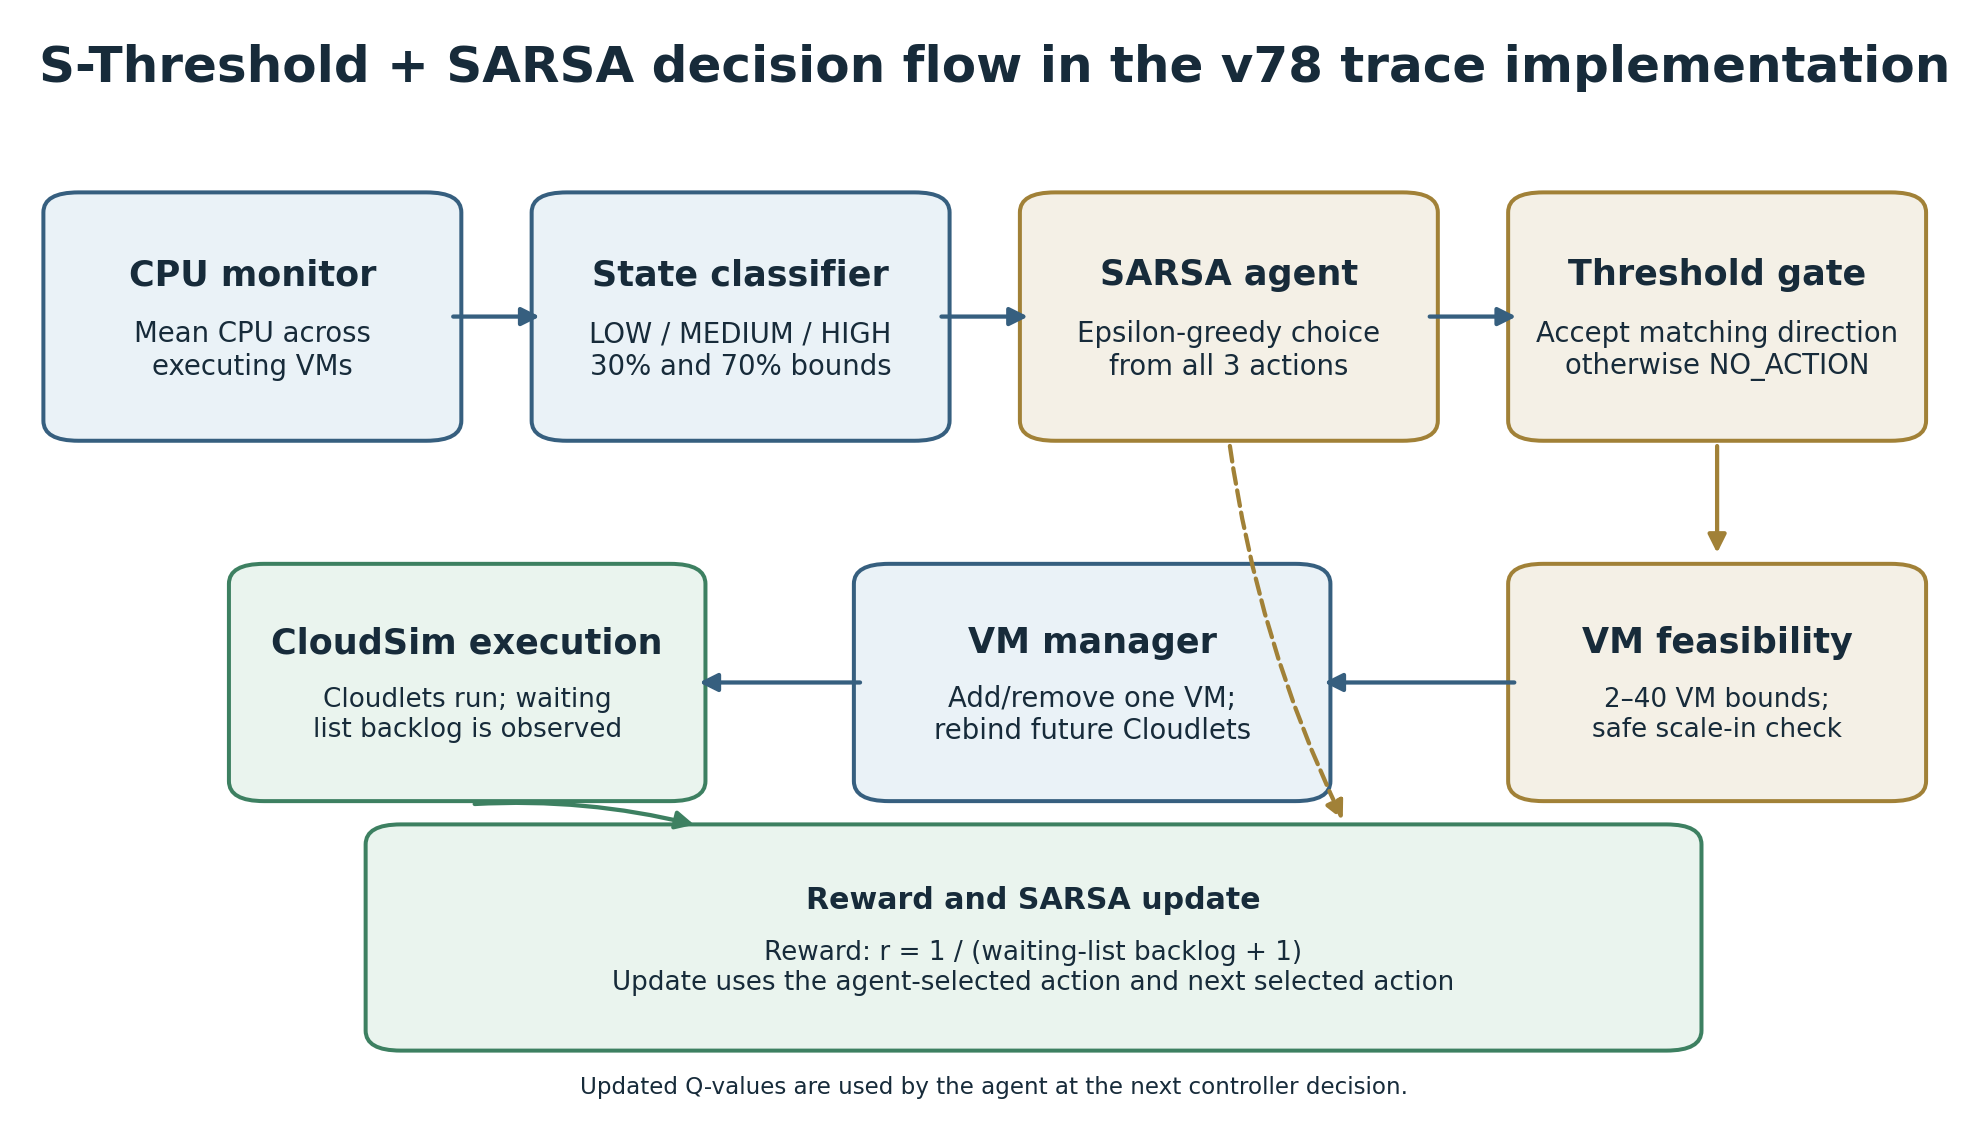
\includegraphics[width=0.98\textwidth]{sarsa_controller.png}
\caption{S-Threshold+SARSA trace-controller flow in the v78 implementation. The agent first selects from all three actions; a separate threshold gate and VM-feasibility checks determine whether a VM operation is applied. The SARSA transition retains the agent-selected action and uses the waiting-list backlog reward.}
\label{fig:sarsa}
\end{figure}

\subsection{Q-THRESHOLD stabilization configuration}

The Q-THRESHOLD result configuration is labelled `Q-Threshold-Stabilized-v2'. Its recorded settings include an exponential moving-average CPU signal with coefficient 0.35; queue-aware scale-out; a requirement for two consecutive scale-out samples and four consecutive scale-in samples; threshold adjustment every 30 seconds; a 10-second minimum action gap; and a 45-second hold before scale-in after a confirmed scale-out, and a 45-second retry backoff after VM-allocation failure. The Q-table and threshold state persist across the three within-day runs and across days. The learning parameters recorded for this run are $\alpha=0.1$, $\gamma=0.9$, and $\epsilon=0.1$.

The Q-THRESHOLD reward is documented in its run configuration as a project-level reward combining response-time and VM-count information. It is distinct from the waiting-backlog reward used by the S-Threshold v78 trace runner and is not claimed to reproduce the exact reward of the S-Threshold paper. The supplied `QThreshold-CloudSim-Plus-30Day-Stability-Fix` source archive contains the stabilizing mechanisms listed above and its settings match the result signature. The historical result package does not preserve an executable hash or source commit identifier, so this remaining provenance limitation should be acknowledged.

\subsection{Experimental protocol}

The same 8,640-step offered-load sequence and the same CloudSim infrastructure settings are used for all four modes. The STATIC mode uses ten VMs. The other modes may change the VM count within the range from two to forty. The S-Threshold batch includes three sequential SARSA trials per day that share a continuing Q-table; these trials are not independent repetitions. The Q-THRESHOLD run also records three runs per day with controller state persisting between runs and across days. We therefore treat the daily aggregate, rather than each within-day run as an independent day, as the unit for descriptive summary statistics.

A day is included only when the batch validation marks it valid. The S-Threshold summary contains 30 valid days and no invalid days. The Q-THRESHOLD summary likewise contains 30 valid days and no invalid days. The per-day means are then summarized across the 30 days using the mean and sample standard deviation. For S-Threshold versus threshold-only, a paired daily difference is also reported because both modes receive the same day's offered-load sequence. We do not conduct inferential significance testing in this version of the study; all comparisons are descriptive.

\subsection{Performance metrics}

The following metrics are used:
\begin{itemize}[leftmargin=1.5em]
  \item \textbf{Average response time}: mean Cloudlet completion time minus arrival/submission time, measured in CloudSim seconds.
  \item \textbf{P95 response time}: the 95th percentile of individual Cloudlet response times within a run.
  \item \textbf{Average waiting time}: mean time from a Cloudlet's arrival until it begins execution.
  \item \textbf{Makespan}: total simulated time required to finish the submitted Cloudlets.
  \item \textbf{Throughput}: number of completed Cloudlets divided by makespan, in Cloudlets per simulated second.
  \item \textbf{Average VM count}: time-averaged number of active VMs.
  \item \textbf{VM-seconds}: the accumulated active VM count multiplied by elapsed simulated time. This is a proxy for VM resource-time consumption.
  \item \textbf{Scaling flaps}: number of reversals between consecutive applied scaling directions (scale-out followed by scale-in, or vice versa).
\end{itemize}

These measures cover service latency, work completion, resource use, and scaling stability. They do not represent monetary cost or energy consumption because neither VM billing prices nor host power models are included in the reported trace experiment.

\begin{figure}[t]
\centering
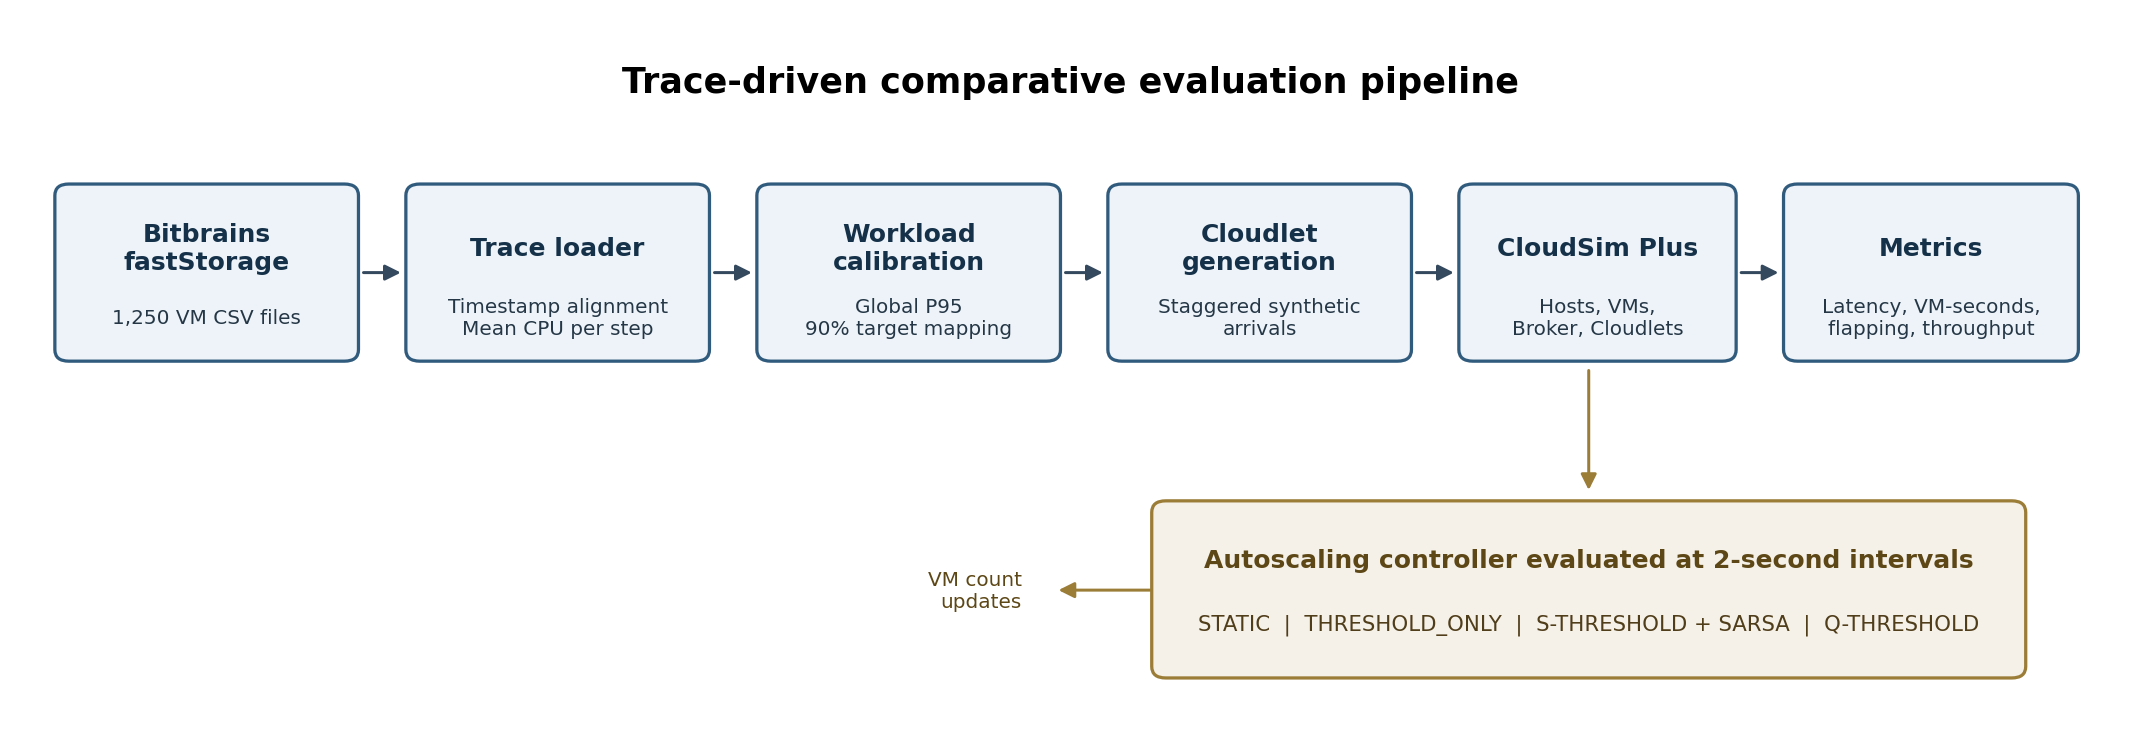
\includegraphics[width=0.93\textwidth]{workflow.png}
\caption{End-to-end trace-driven experimental pipeline. The source trace is transformed into a common synthetic Cloudlet workload, which is executed under each controller mode in CloudSim Plus.}
\label{fig:workflow}
\end{figure}

\section{Implementation Overview}\label{sec:implementation}

The implementation is organized into a trace-preparation layer, a simulation layer, controller components, and a batch-evaluation layer. `BitbrainsTraceLoader` reads the per-VM CSV files, discovers the required timestamp and CPU columns, aligns samples into time buckets, and creates the aggregate CPU time series. `TraceBatchRunner` calculates the global P95 scale factor, divides the trace into daily windows, stores run settings, validates completed days, and manages checkpointed progress. The SARSA Q-table is saved with the batch outputs so that the sequential learning process can be inspected and resumed.

`CloudEnvironment` creates the CloudSim Plus simulation and datacenter. `HostManager` defines the physical hosts. `VmManager` creates VMs and enforces the configured minimum and maximum. `CloudletManager` converts trace-derived offered load into staggered Cloudlet arrivals while carrying fractional arrival counts across windows. `TraceBenchmarkRunner` executes the selected controller mode, monitors VM CPU utilization, schedules controller decisions, measures completed tasks, and records the decision timeline.

For S-Threshold+SARSA, `SThresholdManager` classifies CPU states and applies the threshold gate to the action selected by `SarsaAgent`. `SarsaAgent` maintains the tabular action values, performs epsilon-greedy selection over the three scaling actions, and applies the on-policy SARSA update. `RewardManager` returns the reciprocal of its numeric input; in the v78 trace path the caller passes the broker waiting-list size plus one, so the effective reward is the reciprocal waiting-backlog reward in Eq.~\ref{eq:reward}. `TraceBenchmarkRunner` retains the pending state, agent-selected action, and reward between controller observations. It does not replace the selected SARSA action with the threshold-gated or physically applied action when updating the Q-table.

The Q-THRESHOLD experiment is supplied as a separate stabilized-v2 source package. Its trace runner and controller implement the recorded EMA filtering, queue-aware scale-out, consecutive-sample confirmation, minimum action gap, scale-in hold, and allocation-failure retry behavior. The source archive's settings correspond to the stabilized-v2 result signature. The historical outputs do not contain a build hash or commit identifier, which limits retrospective verification of the exact executable used.

The full 30-day trace experiment is launched through the batch runner, not solely through the demonstration entry point. The project also contains controller demonstrations and a separate synthetic parameter-sweep benchmark; those paths are not mixed into the 30-day trace results reported here. The reported figures and tables are based on the supplied validated 30-day trace result summaries.

\section{Results}\label{sec:results}

\subsection{Validity and overall comparison}

All 30 planned days were marked valid for the S-Threshold batch, and all 30 were marked valid for Q-THRESHOLD. The Q-THRESHOLD daily files record the requested and completed Cloudlet counts and show zero lost Cloudlets in the inspected run outputs. For the S-Threshold batch, the aggregator validates the expected run records and Cloudlet completion before including a day. The reported means and sample standard deviations are computed over the 30 valid daily aggregates.

Table~\ref{tab:results} presents the main results. The STATIC controller has a mean response time of 4.960 seconds and a P95 response time of 12.142 seconds. All three adaptive modes achieve mean response times close to 1.6 seconds. S-THRESHOLD\_SARSA has the lowest mean response time (1.595 seconds) and the lowest mean P95 response time (2.193 seconds). Q-THRESHOLD has a mean response time of 1.610 seconds and P95 response time of 2.237 seconds. Thus, the latency differences among the adaptive modes are small compared with the difference between the adaptive modes and the static baseline.

\begin{table}[!ht]
\caption{Thirty-day trace-driven results (mean $\pm$ sample standard deviation across valid daily aggregates). Times are CloudSim seconds; throughput is in Cloudlets/s. The SARSA column denotes S-THRESHOLD+SARSA.}
\label{tab:results}
\centering
\scriptsize
\setlength{\tabcolsep}{0.5pt}
\begin{tabular}{@{}>{\raggedright\arraybackslash}p{0.19\textwidth}*{4}{>{\centering\arraybackslash}p{0.20\textwidth}}@{}}
\toprule
Metric & STATIC & THRESHOLD & SARSA & Q-THR \\
\midrule
Avg response (s) & $4.9599\pm10.6295$ & $1.5950\pm0.0069$ & $1.5945\pm0.0072$ & $1.6095\pm0.0124$ \\
P95 response (s) & $12.1422\pm27.4718$ & $2.2002\pm0.0273$ & $2.1929\pm0.0246$ & $2.2367\pm0.0717$ \\
Avg waiting (s) & $3.5516\pm10.6282$ & $0.1886\pm0.0041$ & $0.1881\pm0.0056$ & $0.2007\pm0.0169$ \\
Avg VMs & $10.000\pm0.000$ & $13.306\pm4.168$ & $13.538\pm4.021$ & $12.785\pm3.933$ \\
VM-sec. ($\times 10^3$) & $28.84\pm0.13$ & $38.34\pm12.01$ & $39.01\pm11.58$ & $36.84\pm11.33$ \\
Makespan (s) & $2884.60\pm12.99$ & $2881.21\pm0.11$ & $2881.29\pm0.40$ & $2881.25\pm0.16$ \\
Throughput & $3.9099\pm1.2510$ & $3.9164\pm1.2601$ & $3.9163\pm1.2602$ & $3.9164\pm1.2601$ \\
Flaps/day & $0.000\pm0.000$ & $15.333\pm16.352$ & $10.722\pm9.321$ & $2.722\pm3.422$ \\
\bottomrule
\end{tabular}
\end{table}

\subsection{Latency comparison}

Figure~\ref{fig:latency} compares average and P95 response time. STATIC exhibits markedly higher latency and high day-to-day dispersion. Its fixed ten-VM pool cannot respond to workload variation. The adaptive controllers maintain a larger average active VM count and reduce the response-time metrics. The difference between THRESHOLD\_ONLY and S-THRESHOLD\_SARSA is small in their overall means: the SARSA controller's average response time is approximately 0.00044 seconds lower, and its P95 response time is approximately 0.00733 seconds lower. These absolute differences are small relative to the overall response-time scale and should not be described as a large latency improvement.

Q-THRESHOLD's average response time is approximately 0.015 seconds higher than that of S-THRESHOLD\_SARSA, corresponding to roughly 0.94\% relative to the SARSA mean. Its P95 response is approximately 0.044 seconds higher, or about 2.0\%. This suggests a modest latency cost associated with the more conservative behavior observed for Q-THRESHOLD. The results do not establish statistical significance, and the controller runs share sequential learning state; the values are reported as descriptive experiment outcomes.

\begin{figure}[t]
\centering
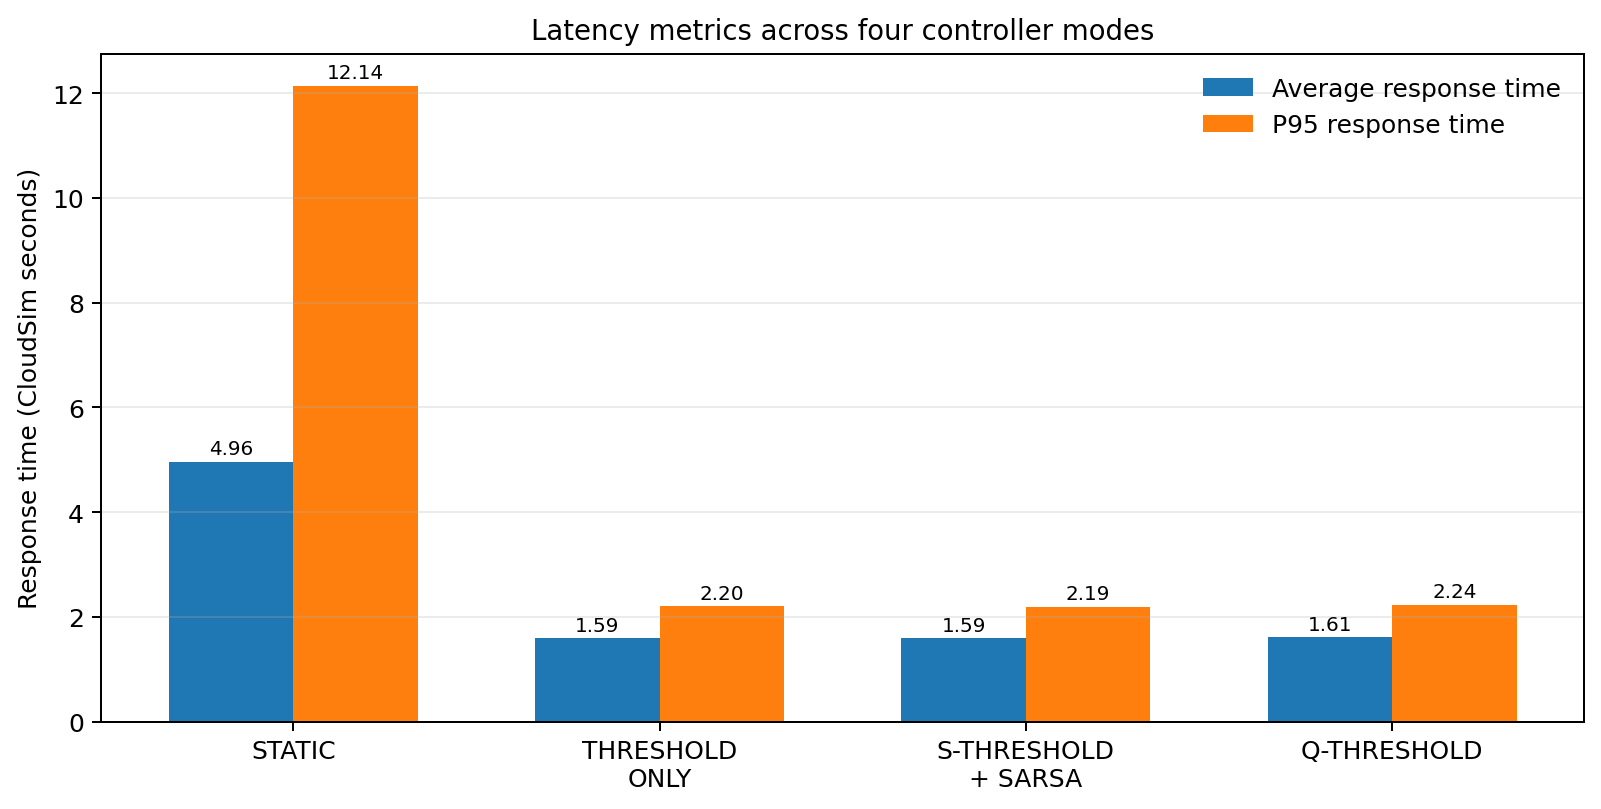
\includegraphics[width=0.88\textwidth]{latency_comparison.png}
\caption{Mean average and P95 Cloudlet response times for the four controller modes. Exact dispersion values are provided in Table~\ref{tab:results}.}
\label{fig:latency}
\end{figure}

\subsection{Resource use and scaling stability}

Figure~\ref{fig:resource} summarizes the active-VM, VM-second, and scaling-flap comparison. Resource use and scaling stability show a different ordering from latency. STATIC has the lowest VM-seconds because it always uses ten VMs, but its response time is much higher. Among the adaptive methods, Q-THRESHOLD has the lowest mean VM count (12.785) and VM-seconds (36,836.6). This is approximately 5.56\% fewer VM-seconds than S-THRESHOLD\_SARSA and 3.91\% fewer than THRESHOLD\_ONLY. The difference indicates that Q-THRESHOLD maintained a smaller average pool over the evaluated workload while keeping latency close to the other adaptive policies.

Flapping is where Q-THRESHOLD exhibits the largest separation. It averages 2.72 scaling-direction reversals per day, compared with 10.72 for S-THRESHOLD\_SARSA and 15.33 for THRESHOLD\_ONLY. Relative to S-THRESHOLD\_SARSA, this is a reduction of approximately 74.6\%; relative to THRESHOLD\_ONLY, it is a reduction of approximately 82.2\%. These reductions are consistent with the smoothing, confirmation, action-gap, and hold settings implemented in the supplied stabilized-v2 source. However, the experiment does not include an ablation of these mechanisms, so their individual causal contributions cannot be isolated from the aggregate comparison.

\begin{figure}[t]
\centering
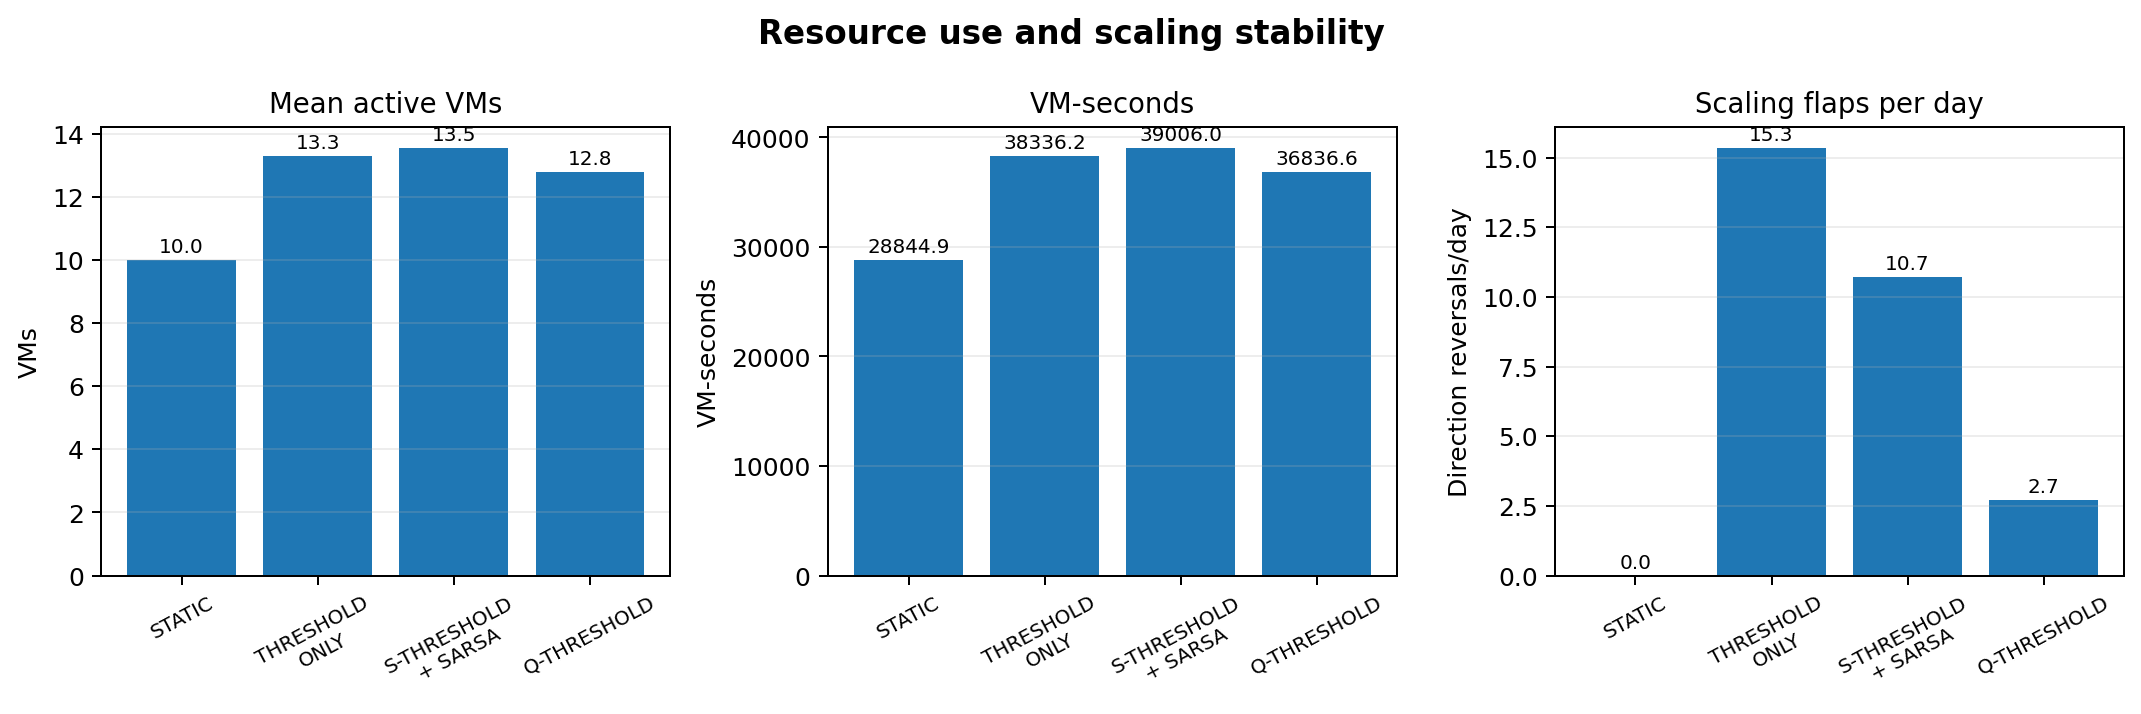
\includegraphics[width=0.95\textwidth]{resource_flapping.png}
\caption{Mean active VMs, VM-seconds, and scaling-direction reversals per day. Q-THRESHOLD records the lowest resource-time use and lowest flapping among the adaptive modes.}
\label{fig:resource}
\end{figure}

\subsection{Makespan and throughput}

The makespan values for the three adaptive modes are close to one another: approximately 2,881.2--2,881.3 simulated seconds. Throughput is also almost indistinguishable across the adaptive controllers, at approximately 3.916 Cloudlets per simulated second. STATIC has a slightly longer mean makespan (2,884.6 seconds) and a mean throughput of approximately 3.910 Cloudlets per simulated second. These values indicate that the adaptive controllers do not produce a material throughput separation in this experiment, even though they differ in response time, resource-time use, and flapping.

The throughput definition used here is completed Cloudlets divided by makespan. It should not be compared directly with a different throughput equation unless the denominator and task-counting convention are the same. The base paper reports its own throughput metric and synthetic benchmark settings \cite{archana2025sthreshold}; the present trace experiment uses staggered synthetic Cloudlet arrivals generated from the Bitbrains trace and therefore has a different workload construction.

\subsection{Paired S-THRESHOLD\_SARSA versus THRESHOLD\_ONLY comparison}

Table~\ref{tab:paired} summarizes the paired daily differences. The S-Threshold batch stores paired daily outcomes for THRESHOLD\_ONLY and S-THRESHOLD\_SARSA under the same offered-load sequence. The mean daily difference for average response time is $-0.000439$ seconds, and the mean daily difference for P95 response time is $-0.007326$ seconds, with negative values indicating lower values for SARSA. The SARSA mode has a lower average response time on 19 of the 30 days and a lower P95 response on 18 days. It also has fewer flaps on 21 days, with a mean reduction of 4.611 flaps per day. On the other hand, it consumes an average of 669.8 additional VM-seconds per day relative to threshold-only, and its average VM count is higher by approximately 0.232. These paired results indicate that, in this configuration, SARSA slightly improves the response-time metrics and reduces direction reversals relative to threshold-only, with a modest increase in resource-time use.

\begin{table}[t]
\caption{Paired daily difference for S-THRESHOLD\_SARSA minus THRESHOLD\_ONLY. Negative values indicate lower values for S-THRESHOLD\_SARSA.}
\label{tab:paired}
\centering
\scriptsize
\setlength{\tabcolsep}{3pt}
\begin{tabular}{lrrrr}
\toprule
Metric & Mean diff. & SD & SARSA lower & Equal/higher \\
\midrule
Avg response (s) & $-0.000439$ & 0.005532 & 19 & 1 / 10 \\
P95 response (s) & $-0.007326$ & 0.029192 & 18 & 2 / 10 \\
Avg waiting (s) & $-0.000540$ & 0.005456 & 19 & 1 / 10 \\
Makespan (s) & $+0.078347$ & 0.394684 & 7 & 11 / 12 \\
VM-seconds & $+669.845$ & 1458.058 & 13 & 1 / 16 \\
Avg VMs & $+0.232250$ & 0.506194 & 13 & 1 / 16 \\
Flaps/day & $-4.611111$ & 14.263552 & 21 & 5 / 4 \\
\bottomrule
\end{tabular}
\end{table}

\subsection{Summary of the observed trade-off}

The results answer the research questions as follows. For RQ1, the adaptive controllers reduce response time substantially relative to the static pool, while the three adaptive modes produce very similar throughput and makespan. For RQ2, S-THRESHOLD\_SARSA has fewer mean daily flaps than THRESHOLD\_ONLY and slightly lower response-time metrics, but it uses somewhat more VM-seconds. For RQ3, Q-THRESHOLD records lower VM-seconds and fewer scaling reversals than S-THRESHOLD\_SARSA, with slightly higher response time. The experiment therefore supports a trade-off interpretation: the SARSA controller is marginally latency-oriented in these results, while the recorded Q-THRESHOLD variant is more resource-conservative and stable.

\section{Discussion}\label{sec:discussion}

\subsection{Interpretation of the controller comparison}

The static baseline demonstrates the consequence of keeping the resource pool unchanged while the workload varies. Although STATIC has the smallest VM-seconds among all modes, this resource saving is accompanied by substantially higher mean response time, P95 response time, and waiting time. The result illustrates why resource usage should not be optimized in isolation. A controller that minimizes the number of VMs may do so at the expense of service performance.

Threshold-only scaling provides a strong improvement over STATIC in the measured response-time metrics. This is consistent with the direct purpose of threshold control: add VMs when utilization crosses a high threshold and remove VMs when utilization falls below a low threshold. However, reactive decisions can reverse direction as measured CPU crosses the configured boundaries. In the evaluated trace, THRESHOLD\_ONLY shows the highest flapping rate among the adaptive methods.

S-THRESHOLD\_SARSA adds an action-value learning component while retaining threshold-based constraints. The mean latency improvement over threshold-only is small, but the direction-reversal count is also lower. This is consistent with the implemented two-stage decision path: SARSA selects among three actions, and the threshold gate suppresses a selected action when it does not match the current LOW/HIGH direction. The reward in this trace path is based on waiting-list backlog, so the small observed latency differences should not be attributed to direct response-time reward optimization. At the same time, the observed average VM count and VM-seconds are slightly higher than threshold-only. The controller should therefore not be described as strictly dominating the threshold baseline.

Q-THRESHOLD records the smallest average VM count and the fewest flaps among the adaptive modes. Its response time remains near the other adaptive controllers but is not the lowest. This behavior is aligned with the additional stabilization mechanisms recorded in the experiment configuration: smoothing and confirmation conditions can reduce the chance of acting on transient changes, while a hold interval discourages rapid scale-in after a scale-out. Still, the present data do not isolate the effect of each mechanism. A future ablation study would be required to determine how much each setting contributes.

\subsection{Implications for cloud controller design}

The measured results reinforce the importance of multi-metric evaluation. If an operator evaluates only average response time, the small advantage of S-THRESHOLD\_SARSA over Q-THRESHOLD may appear decisive. If VM-seconds and scaling flapping are also considered, Q-THRESHOLD presents a different advantage. In an operational deployment, the preferred controller would depend on service-level objectives, resource prices, the cost of VM provisioning, and the penalty for instability. The simulation does not contain a monetary billing model or energy model, so it cannot establish which policy has the lowest financial or environmental cost.

The use of a global P95 calibration factor is also important when interpreting the results. It ensures that each controller receives the same offered-load series on a common capacity scale. It does not prove that a 90\% P95 target is the best operating point for a production cloud. Additional experiments at several P95 targets would be needed to understand sensitivity to the calibration choice.

\subsection{Relationship to prior work}

The results should be interpreted as one experimental comparison within the broader auto-scaling literature. The S-Threshold paper introduces a threshold-plus-SARSA approach and reports CloudSim Plus experiments under synthetic parameter variations \cite{archana2025sthreshold}. This work instead extends the project evaluation to a multi-day trace-derived workload and reports additional resource-time and flapping metrics. The Q-learning literature demonstrates that threshold adaptation and resource provisioning can be formulated as learning problems \cite{song2024qlearning}, while AWARE emphasizes practical issues around transfer and safe exploration in production settings \cite{qiu2023aware}. More recent predictive RL work combines forecasting and deep Q-learning to anticipate demand \cite{lipari2025forecast}. These approaches differ in their deployment contexts and experimental workloads; the current results should not be used to rank them directly.

\subsection{Threats to validity}

Several limitations affect the interpretation and generalizability of the results.
\begin{enumerate}[leftmargin=1.8em]
  \item \textbf{Trace-to-workload transformation.} The Bitbrains trace records VM resource measurements, not the exact request stream of an application. The experiment converts aggregate CPU percentages into synthetic Cloudlet arrivals. This transformation preserves a calibrated offered-load pattern but does not recreate original application semantics, per-VM task placement, or service dependencies.
  \item \textbf{Calibration choice.} The global P95 target is set to 90\% of baseline capacity. This value is an experimental design decision. Different target values can change the generated Cloudlet arrival count and potentially the relative controller outcomes.
  \item \textbf{CPU-only state.} The trace-based S-Threshold state uses CPU utilization. Although the source paper discusses CPU and memory, the current trace implementation does not combine CPU and memory into a joint state. Memory and bandwidth utilization in the synthetic Cloudlets are fixed at 10\% and do not serve as changing state variables.
  \item \textbf{Fixed S-Threshold bounds.} The trace implementation uses fixed 30\% and 70\% thresholds. It does not implement a dynamic threshold formula because a fully specified update rule was not available in the reference description.
  \item \textbf{S-Threshold reward and transition semantics.} In the supplied v78 trace runner, the SARSA reward is the reciprocal of the broker waiting-list size plus one, not inverse response time. The Q-table transition retains the agent-selected action even when the threshold gate or a VM feasibility check prevents the corresponding VM operation. These implementation details differ from an executed-action or response-time-reward formulation and must be considered when interpreting the results.
  \item \textbf{Sequential learning trials.} The three S-Threshold trials per day share a continuing Q-table and are sequential learning trials, not independent replications. The Q-THRESHOLD configuration also states that its Q-table and threshold state persist across repetitions and days. Standard deviations are descriptive across daily aggregates and should not be interpreted as variation across independent algorithm replications.
  \item \textbf{Source/build provenance.} The supplied v78 source plus v78-update-2 patch corresponds to the selected S-Threshold result package, and the supplied stabilized-v2 Q-Threshold source contains the mechanisms recorded in its result signature. However, the historical result packages do not preserve executable build hashes or commit identifiers. The S-Threshold settings signature also does not record a random seed; the source initializes its random generator without a fixed seed. Exact stochastic reruns therefore cannot be guaranteed from the archived metadata alone.
  \item \textbf{Simulation realism.} CloudSim Plus is a discrete-event simulator. The simulation does not model production deployment overheads such as VM boot delay, orchestration latency, real network contention, billing variation, or energy consumption in the reported metrics. Results therefore describe the configured simulation, not a production environment.
  \item \textbf{No inferential test.} This version reports means, standard deviations, and paired descriptive daily differences. It does not report confidence intervals, effect-size tests, or statistical significance tests.
\end{enumerate}

\subsection{Future research directions}

A first extension is to vary the global P95 target and the controller decision interval to determine whether the observed ranking is robust to workload calibration and reaction speed. A second direction is to enrich the S-Threshold state with changing memory utilization and queue length, provided that these inputs are measured consistently and the state definition is explicitly specified. A third direction is to conduct a reward ablation, comparing the current waiting-backlog reward with response-time-based and normalized multi-objective rewards that penalize VM-seconds or scaling actions. A fourth direction is to perform controlled ablations of the Q-THRESHOLD stabilization settings (EMA, confirmation samples, action gap, scale-in hold, and allocation-retry backoff), with versioned source and build metadata for each variant. Finally, predictive methods such as workload forecasting combined with deep RL, and production-oriented mechanisms for safe exploration, are promising directions identified in the recent literature \cite{machiraju2026survey,qiu2023aware,lipari2025forecast}. These are proposed future experiments and are not claimed as implemented features of the current project.

\section{Conclusion}\label{sec:conclusion}

This paper has presented a trace-driven CloudSim Plus comparison of four horizontal auto-scaling controller modes: STATIC, THRESHOLD\_ONLY, S-THRESHOLD\_SARSA, and Q-THRESHOLD. The workload was derived from 1,250 Bitbrains fastStorage VM files, aggregated into 8,640 simulated trace steps, and calibrated with a single global P95 reference that maps to 90\% of the ten-VM baseline capacity. The trace-derived offered load was translated into staggered synthetic Cloudlets, and each controller was evaluated over 30 valid daily windows.

The static configuration produced substantially higher response and waiting times than the adaptive controllers. S-THRESHOLD\_SARSA had the lowest mean and P95 response time among the compared modes, although its latency advantage over threshold-only was small. Q-THRESHOLD used fewer VM-seconds and produced fewer scaling-direction reversals than the other adaptive modes, at the cost of slightly higher response time than S-THRESHOLD\_SARSA. Thus, the results reveal a trade-off between latency, resource-time use, and scaling stability rather than a universal winner.

The study's contribution lies in the trace-driven implementation and comparative evaluation, together with explicit reporting of the assumptions needed to translate the reference S-Threshold approach into a simulation. The findings remain specific to the stated CloudSim configuration and trace-to-Cloudlet transformation. Before submission, the team must complete the public repository upload and final repository, citation, and reproducibility checks. The paper reports the archived experiment outputs and states the remaining source/build provenance limitations explicitly.

\section*{Declarations}

\subsection*{Funding}
This research received no external funding.

\subsection*{Competing interests}
The authors declare no competing interests.

\subsection*{Author contributions}
Conceptualization and methodology: Dilshad. Java/CloudSim implementation: Dilshad, Utkarsh, and Saurabh Verma. S-Threshold+SARSA controller implementation: Dilshad and Utkarsh. Q-Threshold controller implementation: Saurabh Verma. Dataset processing and experimental execution: Dilshad, Utkarsh, and Saurabh Verma, following the dataset and experimental direction suggested by Prof. Mohit Sajwan. Results analysis and graph preparation: Dilshad and Saurabh Verma. Research-paper writing and presentation preparation: all three authors.

\section*{Acknowledgements}
The authors express their sincere gratitude to Prof. Mohit Sajwan, Professor of Cloud Computing, for suggesting the use of the Bitbrains dataset and providing guidance on the experimental direction. The authors also acknowledge Bitbrains IT Services Inc. for providing the workload trace and the Grid Workloads Archive for making the GWA-T-12 dataset available. The associated dataset paper is cited as requested by the provider \cite{shen2015bitbrains}.

\subsection*{Data availability}
The GWA-T-12 Bitbrains fastStorage workload trace used in this study was obtained from the Grid Workloads Archive and is publicly available at \url{https://atlarge-research.com/gwa-t-12/}. The fastStorage data comprise the 1,250 VM trace files used to create the aggregate CPU workload in this study. The processed aggregate trace, experiment configurations, and result summaries will be included in the project repository, subject to the dataset provider's distribution terms.

\subsection*{Code availability}
The project source code, experiment configurations, saved result summaries, and figure-generation materials will be made available through a public GitHub repository before submission. The S-Threshold result set is associated with the v78 source archive and the v78-update-2 patch. The Q-Threshold result set is associated with the inspected Q-Threshold-Stabilized-v2 source archive. The historical result files do not include executable build hashes or commit identifiers; this provenance limitation is documented in the manuscript.

\subsection*{Ethics approval}
Not applicable. The study uses anonymized infrastructure workload traces and simulation; it does not involve human participants, human data, or live vertebrate animals.

\subsection*{Consent to participate}
Not applicable.

\subsection*{Consent for publication}
Not applicable.

\bibliography{references}

\end{document}
